This chapter discusses the performance and test results of the presented solution processor, as well as the assignment it self and the work process around it.

\section{Requirements}

The assignment's main requirement, which was to implement a ``simple multi-cycle MIPS architecture''~\cite[p.114]{compendium}, was met.
It was based on a suggested MIPS-like architecture presented in Figure 4.1~\cite[p.115]{compendium} in the course compendium, as was required.
The required instructions (see table \vref{table:required-instructions}) have been implemented for the processor, as well as a vast array of additional and more complex instructions (see figure \vref{table:implemented-instructions}.
The processor was extensively tested at different levels of abstraction in several simulation environments, which was a requirement that was met.
Finally, the processor was to be tested on a hardware platform.
This requirement was not met.

\section{Additional Goals}

\subsection{Industry Standard Best Practices}

Did we meed the goal about conforming to industry standards?
What are the industry standards?

VHDL is a language defined by standards laid forth by IEEE, the Institute of Electrical and Electronics Engineers.
In order to write good VHDL, it is best to use IEEE-sanctioned standard libraries.

\subsubsection{The \texttt{numeric\_std} package~\cite{why-library-numericstd-is-preferred}} \label{sec:numeric-std}

For doing arithmetic operations on logic vectors in VHDL, many resources will suggest using the functionality provided in the packages \texttt{ieee.std\_logic\_arith} and \texttt{ieee.std\_logic\_unsigned}.
These packages are non-standard packages defined by a company called Synopsis, which makes one of the more popular VHDL tool suites.
Synopsis bundles these packages in their tool distributions, which causes a lot of confusion as to whether or not a part of the standard VHDL library.
Unfortunately, because of this, these non-standard packages have enjoyed wide-spread usage amongst VHDL coders.
This is a problem, because different vendors of VHDL tools have begun supply their own versions of \texttt{std\_logic\_arith} and \texttt{std\_logic\_unsigned}.
Of course, as there is no standard governing these packages, the different versions supplied by different versions have begun to diverge, and are not necessarily compatible with each other.

IEEE has countered this problem by defining new standard packages called \texttt{numeric\_std} and \texttt{numeric\_bit}, which implement similar functionality as the unofficial Synopsis packages.
This ensures compatibility across VHDL tools from different vendors.

\texttt{Numeric\_std} has a number of advantages over \texttt{std\_logic\_arith}.
The biggest advantage is that it defines new types for arithmetical logical vectors, \texttt{signed} and \texttt{unsigned}, as opposed to trying to use \texttt{std\_logic\_vector} directly, which is what the Synopsis packages do.
This is an advantage because combining signed and unsigned arithmetic on the same signals becomes a lot easier.
In fact, the Synopsis packages simply assumes all operands are unsigned in all arithmetic operations, which is a bad idea.
A different advantage with the standard packages is that they provide stronger quality assurance through type checking, as they introduce new types.
This is a good thing because it lets developers find bugs earlier, speeding up the development process.

In the solution VHDL code, all arithmetical operations are sanely implemented using \texttt{numeric\_std}.

\subsubsection{Test Coverage}

The solution processor has very good simulation test coverage.
Every custom entity in the solution VHDL code has its own extensive test bench, which uses the custom-made convenience functions from the \texttt{test\_utils} package.
Unfortunately, the solution processor was never tested physically on the FPGA, due to unfortunate prioritization in the design goals for the assignment.

To improve the test coverage, the obvious next step is to load the solution processor onto an FPGA and run the same tests on the physical board.

\subsection{Instruction Set}

A large instruction set was implemented for the solution processor.
Although implementing it was fun, it distracted from the other parts of the assignment.
One of the reasons for originally choosing to implement the full instruction set was to be able to use existing MIPS tools such as compilers, assemblers, etc.
Unfortunately, not enough instructions were implemented for this benefit to kick in.
Ultimately, this design goal did more harm than good for the solution processor.
On the positive side, implementing a large instruction set turned out to be very educational, as it forced the authors to expand the handout framework and make architectural decisions.
It also helped greatly in the process of becoming fluent and proficient in VHDL.

\subsection{Performance}

The presented solution processor performs rather well for a sequential simple multi cycle processor.
The clock's maximum speed is 56.277Mhz \vref{sec:discussion-performance}.
Being a multi-cycle processor, most instructions take more than one cycle to complete.
Instructions that only operate on immediates and registers take two cycles to complete.
Instructions that access the data memory require an additional cycle, for a total of three cycles.
This means that under optimal conditions, the processor is theoretically capable of 26,138,500 instructions per second.

One way of increasing performance beyond what has been done in the solution is to restructure the logical flow of the architecture to keep the data flow dependencies to a minimum.
Doing so would mean that the processor would need less time to stabilize for each cycle, and as an effect, the clock cycle speed could be increased.
As we all remember from Intel and AMD marketing in the early 2000s: more MHz means more power!

To further increase performance, we could introduce instruction-level parallelism in the form of a pipeline.
This, however, is out of the scope of this exercise.

\section{Energy Efficiency}

Any computer-related report worth its salt should contain a section that discusses the energy efficiency of the presented solution.
This report is no different.
The solution processor was not designed with energy efficiency as a primary design goal.
It does, however strive for simplicity in its VHDL design, using official IEEE-recommended industry standards for as many operations as possible.
This lets the synthesizer use its intimate knowledge of the feature set of the target FPGA to create customized hardware configurations that exploit the possibilities the FPGA provides.
This means that dedicated utility slices, block RAM sections and similar will be used where possible.
They are typically faster than their custom logic counterparts, and therefore allow for quicker execution.
Although quicker execution by virtue of increased clock speeds does not change the energy efficiency of the processor for finite terminating programs, it may allow other dependent components in a larger system to enter low energy states quicker, and thereby reducing static energy loss in the system as a whole.

To make the processor more energy efficient, sleep states could be introduced.
They allow the processor to enter low energy states when it is not needed, i.e. typically when it is waiting for an external signal in a larger system, and when it has nothing else useful to do.

Since the solution processor supports a large amount of diverse instructions, it can execute programs in fewer cycles than a simpler processor, because it can combine several simple instructions into a single complex one.
This means that the processor needs to do less work in total, and is more energy efficient.

\section{About the Work Process}

Work began shortly after the assignment's official starting date\footnote{2013-09-10} and the process chiefly consisted of sporadic lab sessions throughout the following weeks.
The frequency of these sessions increased as the deadline approached, see figure \vref{figure:git-activity-01}.
On the last couple of days before the deadline, approximately all our waking time was devoted to finishing the assignment.

\begin{figure}
	\begin{center}
		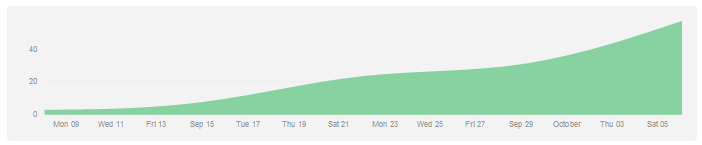
\includegraphics[keepaspectratio, width=\textwidth]{graphics/codebase.PNG}
		\caption{Graph displaying the number of commits to the assignment's code repository on github over time}
		\label{figure:git-activity-01}
	\end{center}
\end{figure}

Shortly after the work began a decision was made to rewrite the ALU from scratch, as using the one included in the assignment files would conflict with our third goal relating to performance (see section \vref{sec:goals-performance}).
While this choice was in accordance with our goals, it was -- strictly speaking -- unnecessary.
The time could have been spent otherwise, perhaps on trying to flash the FPGA.
\textit{However}, inspiration is a fickle mistress: there is never a guarantee that time spent on one task could ``just as well'' have been spent on another.

Flashing the FPGA was given a lower priority than, amongst other things: writing the report, getting the VHDL code to compile, writing testbenches and sleeping.
We reasoned that delivering a solid report would be a more efficient use of our time rather than spending our last hours before the deadline trying to flash the FPGA, and as a result possibly having to deliver a sub-par report.

In retrospect we should probably have increased the effort earlier and tapered it off at a sustainable amount, e.g. \textit{less} than 16 hours a day.
However we are quite satisfied with the outcome, even though we did not meet all of the assignment's requirements.
We've learned a lot and accomplished a whole lot, and trying to navigate the windows tool chain while trying to flash the FPGA was the least enjoyable part of the assignment.

The specifics of each group member's day-to-day varied: two thirds of the group's members kept a log of their work sessions on the project's GitHub wiki. 
The logs vary in content.
Some of them contain the approximate starting time of the work session and nothing else while others contain a detailed description of the challenges and tasks encountered throughout the session.
The ones containing a more detailed description of the day's events and undertaken tasks proved to be valuable resources during the report's design.
